\documentclass[a4,10pt,comentarios]{aleph-notas}
\usepackage{aleph-comandos}
\usepackage{enumitem}
\usepackage{amssymb}
\usepackage{hyperref}
\usepackage{multicol}
\usepackage{amsmath}
\usepackage{graphicx}
\usepackage{listings}
\usepackage{algorithm}
\usepackage[parfill]{parskip}
\usepackage[noend]{algpseudocode}
\usepackage{natbib}
\bibliographystyle{apa}

\fuente{montserrat}
\graphicspath{ {./img/} }
\setlength{\headheight}{44pt}

% -- Datos de la tarea
\institucion{Criptografía y Seguridad}
\autor{Uziel Vidal Cruz Vargas\\
Emilio Arsenio Raudry Rico}
\tema{Práctica 02: Explotación de vulnerabilidades:\\
desbordamiento de búfer.}

\logouno[9cm]{img/fc}
\begin{document}

\encabezado

\section{Introducción}

La seguridad informática es un aspecto crítico en la actualidad, ya que la información es uno de los activos más valiosos de cualquier organización
Las pruebas de penetración, o \textit{pentesting}, son evaluaciones de seguridad diseñadas para identificar vulnerabilidades en sistemas y redes antes de que puedan ser explotadas por actores malintencionados (Mitnick \& Simon, 2002).

En esta práctica, se enfoca la fase de \textbf{recopilación de información}, una etapa esencial del \textit{pentesting} en la que se recolectan datos clave sobre el objetivo para evaluar posibles puntos débiles. 
Para ello, se emplearán diversas herramientas y metodologías que permiten obtener información de manera estructurada y efectiva (Campbell \& Beach, 2016).

Este documento presenta los requisitos, las fuentes de información utilizadas, el proceso de adquisición de datos, el procesamiento de la información obtenida, el análisis de resultados y una serie de preguntas clave relacionadas con la seguridad informática y el \textit{pentesting}. 
Finalmente, se ofrecerá una conclusión sobre los hallazgos obtenidos y su relevancia en el ámbito de la ciberseguridad.

\bibliographystyle{apa}
\bibliography{referencias}

\section{Recopilación}

Cada uno de los dos programas cuenta con una función la cual solo es accesible si ingresamos una contraseña correcta. Nuestra prueba consiste en probar lo opuesto, demostrar que podemos acceder a dichas funciones (y la información que estas contienen) sin necesidad de si quiera usar las contraseñas.

Al tratarse de una prueba de caja blanca, contamos ya con el código fuente, el cual nos servirá para que sepamos qué direcciones de memoria acceder más adelante. Para el punto anterior nos apoyaremos en la herramienta GDB.

Como nuestro ataque será mediante un buffer overflow, también necesitaremos una herramienta con estructuras de flujo iterativas como python3.

Finalmente, como tratamos con un tipo de ataque altamente conocido y tratado a lo largo de los años, partiremos de que la aleatoriedad de espacio de direcciones virtuales en el kernel de Linux se encuentra desactivado. Esto lo podemos lograr con el comando:

\begin{center}
    \texttt{sudo sysctl -w kernel.randomize\_va\_space=0}
\end{center}
\section{Análisis}
Retomando nuestros apartados durante la adquisición y el procesamiento, filtraremos nuestros resultados de la misma manera.

\subsection{unam.mx}

\begin{enumerate}
    \item Direcciones y dominios:
        Todo correcto.
    \item Fechas importantes: Expira este mes.
    \begin{enumerate}
        \item Creación:1989-03-31
        \item Actualización: 2024-03-27
        \item Expiración:25-03-30
    \end{enumerate}
    \item Datos de la organización: Además de obtener los datos de la UNAM incluye el nombre del servidor intermedio durante el recorrido hasta el servidor objetivo.

    \item Conectividad: Conexión correcta

    \item Información de Red y DNS: Varias subredes, valdría la pena verificar ellas también. Los subdominios nos hablan de contactos para ingeniería social y otros servicios que ofrece la universidad.

    \item Información de puertos, servicios y sistema operativo
        
        \begin{enumerate}
            \item Puertos y servicios: Puerto http abierto, sin cifrado, si alguien se conectara dentro de una red cercana podríamos obtener sus datos en bruto. También podíamos ver que subrutas hay dentro de la página en búsqueda de un archivo perdido con información valiosa.
            \item Usa un sistema Linux, tiene una forma especial de subir de privilegios.
        \end{enumerate}
\end{enumerate}

\subsection{ipn.mx}
\begin{enumerate}

    \item Direcciones y dominios: Todo correcto
    \item Fechas importantes: Expira el año siguiente.
    \item Datos de la organización: Esta administrado por un servidor remoto Microsoft en Estados Unidos. En caso de querer hacer ingeniería social sobre los trabajadores hay que contemplar el lenguaje y el perfil de los usuarios que aparentemente varían de etnias.

    \item Conectividad: Conexión correcta.

    \item Información de Red y DNS: Varias subredes y subdominios. Uno de gran interés es el backup.
    \item Información de puertos, servicios y sistema operativo: A pesar de lo que dice la aproximación de SO, tcpwrapper es un protocolo usado en distribuciones GNU/Linux.

\end{enumerate}

\subsection{pemex.com}

\begin{enumerate}
    \item Direcciones y dominios: Todo correcto

    \item Fechas importantes: Expira el siguiente año.
    \item Datos de la organización: Forma parte del gobierno mexicano. Dentro del personal se encuentran dos personas que aparentemente son parientes (hermanos), implicando un vínculo personal.

    \item Conectividad: Conexión adecuada.

    \item Información de Red y DNS: Varias subredes, al igual muchos servicios varios. Dentro de los subdominios se encuentran contactos con el personal.

    \item Información de puertos, servicios y sistema operativo
        
    \item Puertos y servicios:A pesar de lo que dice la aproximación de SO, tcpwrapper es un protocolo usado en distribuciones GNU/Linux.

\end{enumerate}


\subsection{gob.mx}

No hay dirección IP en un servidor DNS autorativo.
\section{Explotación}

Dado que ambos códigos hacen uso de una función considerada peligrosa, por lo que para poder compilarlo tendremos que proveerle a \textit{gcc} ciertas banderas:

\begin{quote}
\texttt{gcc -g -fno-stack-protector -z execstack nombreCodigo.c -o nombreCodigoCompilado -std=c99 -D\_FORTIFY\_SOURCE=0}
\end{quote}

\begin{center}
    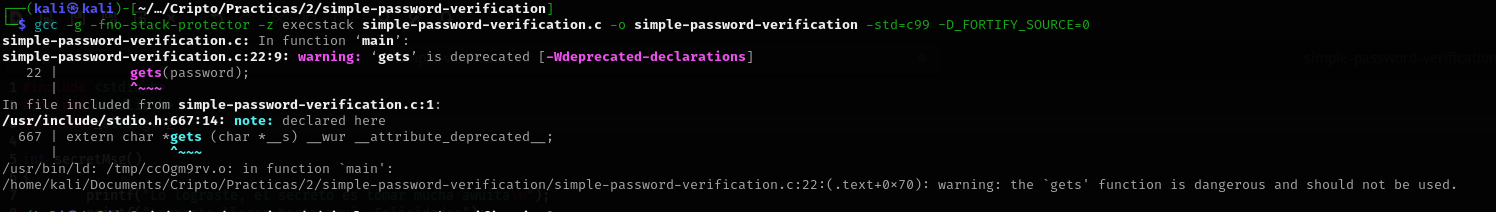
\includegraphics[scale=.3]{img/compilePassword.png}
\end{center}

\begin{center}
    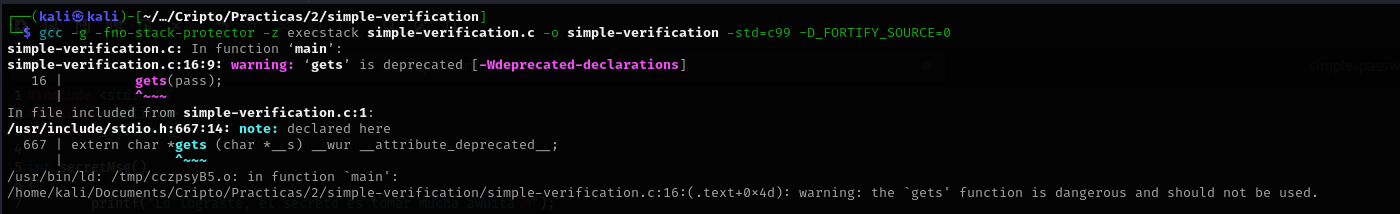
\includegraphics[scale=.3]{img/compileVerification.png}
\end{center}

Estas nos permiten indicarle al compilador lo siguiente:

\begin{itemize}
  \item \texttt{-g} Hace que el compilador incluya información de depuración que necesitaremos cuando usemos a GDB.
  \item \texttt{-fno-stack-protector} Hace que se desactive la protección del stack.
  \item \texttt{-z execstack} Hace que se pueda ejecutar código en el stack.
  \item \texttt{-std=c99} Establece el estándar C99.
  \item \texttt{-D\_FORTIFY\_SOURCE=0} Desactiva las optimizaciones de seguridad en las funciones de manejo de cadenas y buffers.
\end{itemize}

Una vez compilado el programa podemos ejecutarlo con GDB.

Lo ejecutamos de forma depurada con el comando \texttt{start}.

En el primer código, deseamos acceder a la función \texttt{granted()}, por lo que debemos de buscar su ubicación dentro del stack. Para ello podemos usar el siguiente comando de GDB \texttt{print granted}:

Hacemos lo mismo para el segundo código, donde el nombre de la función que buscamos es \texttt{secretMsg()}, ejecutando así en GDB \texttt{print secretMsg}:

\begin{center}
    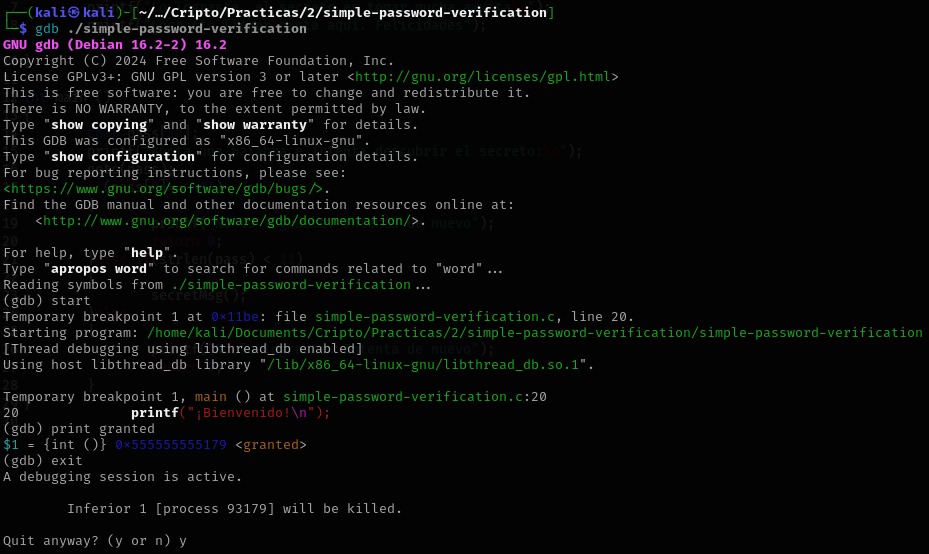
\includegraphics[scale=.5]{img/gdbPassword.png}
\end{center}

\begin{center}
    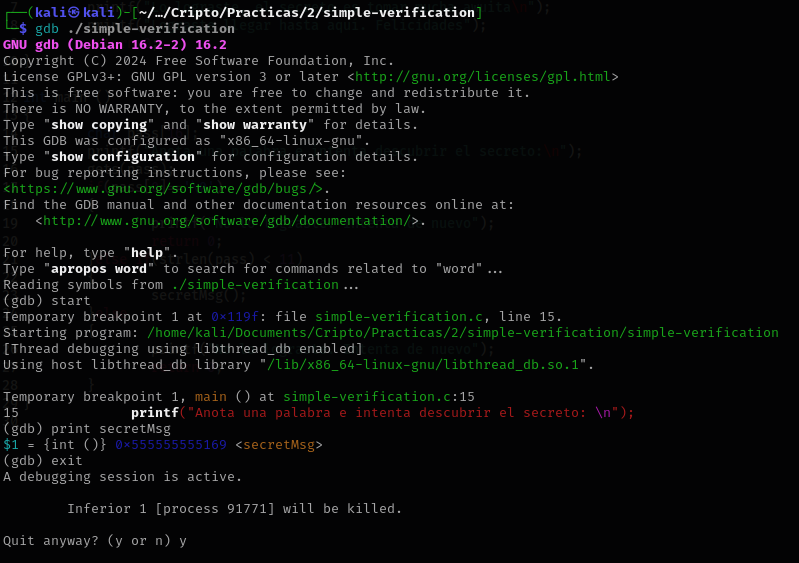
\includegraphics[scale=.5]{img/gdbVerification.png}
\end{center}

Anotamos las direcciones de ambas y salimos de GDB. El motivo de esto, es que, una vez que llenemos el buffer con su máxima capacidad, podamos escribir en el registro de dirección de retorno del stack, la dirección de memoria de dichas funciones.

De esta manera, nuestro exploit consistirá en una entrada de tipo string compuesta por una cantidad caracteres igual al límite del buffer concatenados con la dirección de memoria de ambas funciones. 

Una observación importante es que al momento de que la computadora lea la dirección de memoria, esta debe de estar en formato little endian, la cual consiste en dividir la dirección original en parejas de caracteres y añadirlos en una cadena en orden inverso, donde cada pareja le preceden los caracteres \texttt{\textbackslash x}.

Para realizar estos nos apoyaremos de python, de manera que nuestro exploit se ejecute bajo el siguiente comando:

\begin{quote}
\texttt{python3 -c 'print(''A''*\{límite del buffer\} + "[dirección de memoria de la función]") | ./[nombre del programa compilado]'}
\end{quote}


La bandera \texttt{-c} permite ejecutar python3 desde la línea de comandos. Hacemos que imprima una cantidad de caracteres igual al límite del buffer (en este caso usaremos a la letra A), y le concatenamos la dirección de la función en little endian. Dicha salida se la pasamos a nuestro programa para que la reciba como entrada al momento de ejecutarse.

Al momento de probar el exploit, intentamos con 16 A's (pues el es el tamaño de los dos arreglos que contienen nuestra entrada en los códigos), al no bastar les incrementamos uno hasta llegar al número 24.

De manera que para el primer código, el exploit quedó de la siguiente manera:

\begin{quote}
\texttt{python3 -c 'print(''A''*24 + "\textbackslash x79\textbackslash x51\textbackslash x55\textbackslash x55\textbackslash x55\textbackslash x55") | ./simple-password-verification'}
\end{quote}

\begin{center}
    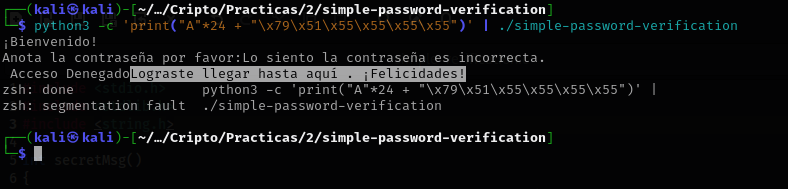
\includegraphics[scale=.5]{img/exploitPassword.png}
\end{center}

Mientras que para el segundo código, quedó así:

\begin{quote}
\texttt{python3 -c 'print(''A''*24 + "\textbackslash x69\textbackslash x51\textbackslash x55\textbackslash x55\textbackslash x55\textbackslash x55") | ./simple-verification'}
\end{quote}

\begin{center}
    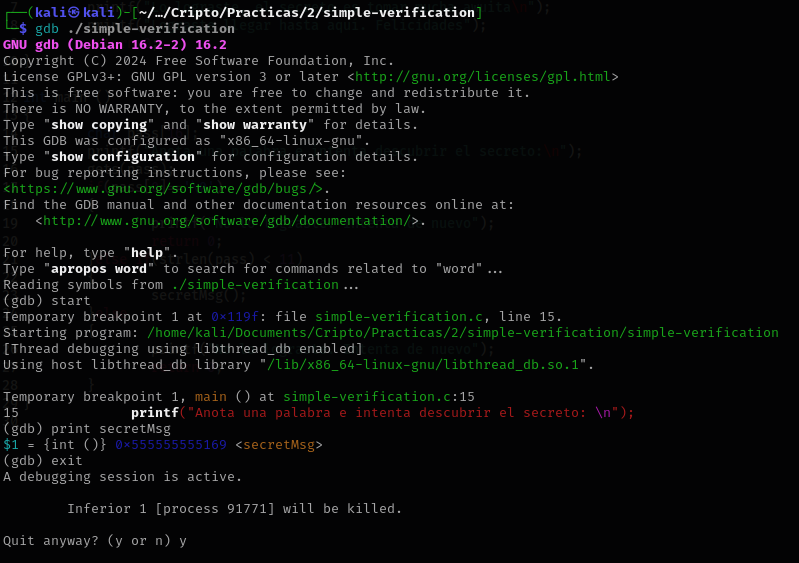
\includegraphics[scale=.5]{img/gdbVerification.png}
\end{center}

Podemos ver que en ambos casos, se pudo acceder a la función adecuada, pues recibimos los mensajes de aceptación.
\section{Post-explotación}

Lo que hicimos básicamente fue darle de entrada a los programas una cadena compuesta por dos partes. La primera subcadena consistió en una cantidad de letras \texttt{A} lo suficientemente grande para poder llenar el espacio designado en el stack al buffer. La segunda subcadena consistía en la dirección de la función a la que buscamos acceder.

El exploit es capaz de llevarnos a la ejecución de dicha función, pues dentro del stack, el bloque del buffer se encuentra justo al lado del bloque de la dirección de retorno. Esto hace que al momento de acceder a dicho bloque, en lugar de volver a la dirección de retorno de la llamada inicial, nos lleve a la que nosotros pusimos.

De esta manera, en ambos casos llegamos los bloque de código que queríamos sin tener que poner las contraseñas requeridas.

Para poder mejorar la seguridad del código, de entrada, no hay que usar funciones de bajo nivel tan inseguras como \texttt{gets()}. Siendo preferibles el uso de otras funciones para recibir entradas, como lo es \texttt{fgets()}. El cual comprueba el tamaño de la entrada para evitar desbordamientos.

No obstante, el mejoramiento no se debe limitar únicamente a eso. 

El primer código hace una llamada al sistema directamente, el cual, tras esta práctica acaba de demostrar lo peligroso que es esto, pues abre una ventana para poder modificar todo el sistema. (Es incluso por esta razón, el porqué no es recomendable darle a lenguajes de programación, la posibilidad de ser ejecutados como root por cualquier usuario).

Otra opción es la inclusión de control de errores, ya que, a pesar de tener métodos seguros, es mejor establecer una lógica robusta que ni siquiera le de la oportunidad al usuario de alcanzar casos críticos.

Otro añadido, que debería considerar más por convención que por otra cosa, es que al momento de hacer las verificaciones de las contraseñas, estas no se hagan en texto plano, si no bajo un hasheo. Esto tampoco es enteramente seguro, pues pude haber ataques de diccionario o fuerza bruta, pero impide una presencia explícita de la contraseña en el código.
\section{Alcance}
El alcance de un desbordamiento de buffer es igual de amplio que el alcance que pude tener la función a la que queramos acceder desde su dirección en el  \texttt{stack}.

En la función \texttt{granted()} (que accedimos en el primer código) hay una línea que abre la terminal de gnome (aunque por la configuración de nuestra máquina virtual, esta no se pudo abrir). Lo que nos puede permitir hacer modificaciones en el sistema e incluso, la posibilidad de escalar privilegios para poder hacer todo lo que queramos siendo root.

También puede ser que la función a la que llamemos, nos permita acceder información sensible, como lo fue con \texttt{secretMsg()}, que podamos robar, o incluso ocupar después para hacer movimientos laterales o causar mayores daños.
\section{Preguntas y Respuestas}

\begin{enumerate}

    \item \textbf{¿Qué significa que una prueba de penetración sea de caja blanca?}

    Una prueba de penetración de \textit{caja blanca} implica que el evaluador tiene acceso total
    al conocimiento del sistema o aplicación a probar, incluyendo código fuente, configuraciones,
    arquitectura de software, credenciales, etc. En esta práctica, contamos con el código fuente de
    los programas vulnerables, lo que nos permite comprender en detalle su funcionamiento interno
    y diseñar exploits de forma más directa. (véase \citep{cowan2002}).

    \item \textbf{¿Por qué es necesario aprender a explotar código?}

    Porque comprender cómo se explota el código inseguro permite:
    \begin{itemize}
        \item Identificar y mitigar de manera efectiva las vulnerabilidades.
        \item Validar la seguridad de un sistema, asumiendo el papel de un “atacante ético”.
        \item Crear conciencia sobre la importancia de escribir y mantener código seguro.
    \end{itemize}

    (Como discuten \citet{erickson2008} y \citet{howard2003}).

    \item \textbf{Menciona el significado de los siguientes registros: EAX, EBX, ECX, EDX, ESI, EDI, EBP, ESP, EIP.}

    Estos registros corresponden a la arquitectura x86 (y en versiones extendidas a x86-64, con nombres similares)(\citealp{foster2005}; \citealp{gupta2012}). A grandes rasgos:
    \begin{itemize}
        \item \textbf{EAX (Extended Accumulator Register)}: utilizado generalmente para operaciones aritméticas y como registro de retorno de funciones.
        \item \textbf{EBX (Extended Base Register)}: se emplea a menudo como base para cálculos de direcciones en memoria.
        \item \textbf{ECX (Extended Counter Register)}: se usa como contador en bucles e instrucciones repetitivas.
        \item \textbf{EDX (Extended Data Register)}: apoya a EAX en operaciones aritméticas de mayor tamaño (multiplicaciones y divisiones).
        \item \textbf{ESI (Extended Source Index)}: comúnmente se usa como puntero fuente en operaciones de cadena.
        \item \textbf{EDI (Extended Destination Index)}: análogo a ESI, pero para el destino.
        \item \textbf{EBP (Extended Base Pointer)}: señala el inicio del marco de pila de una función, facilitando acceso a parámetros locales.
        \item \textbf{ESP (Extended Stack Pointer)}: apunta al tope actual de la pila.
        \item \textbf{EIP (Extended Instruction Pointer)}: contiene la dirección de la instrucción que se ejecutará a continuación.
    \end{itemize}

    \item \textbf{¿Qué es \textit{little endian} y \textit{big endian}? ¿Cuál usa mi procesador? ¿Qué arquitectura tiene mi computadora?}

    El \textit{endianess} describe el orden en que los bytes se almacenan en memoria. En 
    \textit{little endian}, el byte menos significativo se almacena en la dirección de memoria 
    más baja; en \textit{big endian} sucede lo contrario.  
    \\
    Mi procesador (x86\_64) emplea \textit{little endian}, que es el formato común en la mayoría 
    de procesadores Intel y AMD de 64 bits en la actualidad.

    \item \textbf{¿Qué es un segmento y qué es un \textit{offset}?}

    En el contexto de las arquitecturas x86 clásicas, un \textit{segmento} es una región 
    lógica de memoria definida por un registro de segmento. El \textit{offset} es el 
    desplazamiento relativo dentro de ese segmento. Con la evolución a x86\_64, la segmentación 
    se redujo, pero estos conceptos se mantienen en la base de la arquitectura \citep{erickson2008}.

    \item \textbf{¿Qué realiza la instrucción \texttt{lea} en ensamblador?}

    La instrucción \texttt{lea} (\textit{load effective address}) carga en un registro la
    dirección efectiva de una operación de memoria en lugar de cargar el valor que reside en 
    esa dirección. Se usa para cálculos de direcciones y puede reemplazar operaciones de suma 
    o aritmética directa sin tocar la memoria \citep{erickson2008, howard2003}.

    \item \textbf{¿Crees que esta vulnerabilidad desapareció con las nuevas funciones seguras como \texttt{fgets}?}

    No. Usar funciones más seguras como \texttt{fgets} reduce la probabilidad de un desborda-
    miento, pero no lo elimina por completo. Las vulnerabilidades de desbordamiento siguen 
    presentes si no hay validaciones de longitud adecuadas o existen otros errores de manejo 
    de memoria. Por tanto, las \textit{buenas prácticas de programación} siguen siendo 
    esenciales para la seguridad.

    \item \textbf{Investiga tres casos famosos en los cuales se explotó la vulnerabilidad de desbordamiento de búffer. ¿Cuáles fueron sus repercusiones?}

    \begin{itemize}
        \item \textit{Morris Worm (1988)}: primer gusano ampliamente difundido, se basó en
              varios exploits (incluyendo el desbordamiento de \texttt{finger}), colapsando
              grandes partes de Internet de aquel entonces \citep{gallagher2014}.
        \item \textit{Blaster Worm (2003)}: atacaba el servicio RPC de Microsoft Windows,
              propagándose masivamente y ocasionando importantes pérdidas económicas \citep{cert2003}.
        \item \textit{Heartbleed (2014)}: vulnerabilidad en la implementación de OpenSSL,
              que si bien no era un \textit{overflow} clásico, explotó la mala validación de
              un búfer para leer datos sensibles de la memoria del servidor \citep{morrisworm2018}.
    \end{itemize}

    \item \textbf{¿Qué es el bug \textit{Off-by-One}? ¿Cómo funciona? ¿Cómo se previene?}

    Es un error en el manejo de índices o límites de un arreglo, en que se accede o sobrescribe 
    un elemento adicional (o se queda corto por uno). Puede provocar desbordamientos 
    inadvertidos y comportamientos inesperados. Para prevenirlo, hay que hacer validaciones 
    apropiadas de los límites y utilizar funciones o métodos que obliguen a especificar la 
    longitud real de los buffers\citep{howard2003}.

    \item \textbf{¿Se podría explotar la vulnerabilidad de desbordamiento de búfer usando Bash? Argumenta tu respuesta.}

    Es posible pasar \textit{inputs} maliciosos desde Bash a programas vulnerables en C 
    (encadenando el ataque). Sin embargo, explotar directamente la memoria del intérprete 
    Bash requeriría un bug interno en Bash escrito en C. Lo más común es usar Bash 
    simplemente como \textit{medio} para inyectar la cadena maliciosa a programas en C 
    propensos al desbordamiento.
    
\end{enumerate}



\bibliography{referencias}

\end{document}